\documentclass[main.tex]{subfiles}
\begin{document}
% neue TOC:
% \begin{itemize}
%     \item DONE wie im konzept gesagt vergleichen wir algorithmen um \$FRAGE zu beantworten
%     \item DONE zunächst definieren wir, wie und woran wir die performanz der algos vergleichen
%     \begin{itemize}
%         \item DONE Wir werden die performanz an 3 metriken messen: P,R,F1 (siehe BG section)
%     \end{itemize}
%     \item wie im konzept festgestellt, sind die pdas nicht vergleichbar. daher haben wir 2 verschiedene datensätze rausgesucht und oder erstellt:
%     \begin{itemize}
%         \item 2D 3D S: statisch, direkt ganze wolke da
%         \item FIN: dynamisch, inkrementell aufbauend
%     \end{itemize}
%     \item wir führen experimente auf beiden datensätzen durch 
%     \item im anschluss werten wir die ergebnisse aus und evaluieren inwiefern die algorithmen echtzeitfähig sind
% \end{itemize}

\chapter{Evaluation}

In diesem kapitel werden zuvor ausgewählte algorithmen einheitlich verglichen und die resultierenden ergebnisse ausgewertet.
\section{Protocol}
% \begin{itemize}
%     \item was wir zeigen wollen
%     \item daher vergleichen wir algorithmen
%     \item wie vergleichen wir, woran ziehen wir schlüsse? 
% \end{itemize}
This work aims to determine which plane detection algorithm is the most suitable for an AR/VR system. For this decision, we uniformly compare the algorithms selected in
Chapter~\ref{chap:Concept}. We split the comparison into two experiments conducted on different datasets: the 2D-3D-S and the
self-created FIN dataset. Since both datasets are fundamentally different, we will perform the experiments and the analysis separately and then compare the results.
First, we present the metrics used for comparison, followed by an outline of the used configurations of parameters for each experiment.
% In this work, we perform a uniform comparison of plane detection algorithms. This comparison aims to evaluate the real-time plane 
% detection on off-the-shelf hardware through the selection of the best algorithm.
% In the following subsection, we present the metrics used for the evaluation.
% We conduct experiments on both datasets and compare the results of both experiments with respect to the real-time applicability of the
% algorithms. Particularly interesting are the differences resulting from the temporal component.
% Finally, by evaluating the results of both experiments, we determine the most suitable plane detection algorithm for real-time, indoor environments. 

\subsection{Metrics}
To quantify the accuracy of the plane detection algorithms, we use the detected planes and the created ground truth to calculate the three following
metrics: Precision, Recall, and the F1-score. The procedure of calculation is taken from~\cite[Section~4]{Araújo_Oliveira_2020} and detailed
in Section~\ref{sec:metrics}.


\textcolor{red}{hier noch mehr ins detail gehen? (antwort) \underline{\hspace{2cm}}}


In addition to the accuracy of an algorithm, we precisely measure the calculation time by splitting the calculation into pre-processing, plane
detection, and post-processing.
RSPD and OPS perform an initial estimation of normals, while 3D-KHT and OBRG construct an octree during their
pre-processing phase. Note that the octree construction of OBRG includes a local estimation of normals on the
leaf level. OPS merges smaller planes if they pass a coplanarity test and then re-estimates the normals of the
resulting plane. In the post-processing step, OBRG refines the borders of detected planes by inserting
previously unallocated regions.
The pre-and post-processing steps are summarized in Table~\ref{tab:pre-post}.

\begin{table}[H]
    \centering
    \begin{tabular}{c|cccc}
             & RSPD        & OPS        & 3D-KHT         & OBRG           \\ \hline
        Pre  & Normal est. & Normal est & Octree constr. & Octree constr. \\
        Post & /           & Merge      & /              & Refinement
    \end{tabular}
    \caption{Pre-processing and post-processing steps of the plane detection algorithms. RSPD and 3D-KHT do not have any post-processing steps.}
    \label{tab:pre-post}
\end{table}


\subsection{Parameterization of Algorithms}
Because the datasets inherit different amounts of noise, it is necessary to modify the algorithms accordingly.
We thereby modify the algorithms' parameterization to achieve more noise robustness.
In the following, the parameterizations of the algorithms with respect to the two experiments are outlined.
Therein, we refer to the parameterization of the 2D-3D-S experiment as the default configuration.
All deviations from this default configuration necessary for the FIN experiment are determined empirically.


\subsubsection{RSPD}
\textbf{\textcolor{red}{die abkürzungen werden sicherlich im BG erklärt.}}
\begin{table}[H]
    \centering
    \begin{tabular}{c|cccccc}
        Experiment & $l_O$ & $\varepsilon$ & MOR  & $k$ & MND & MDP   \\ \hline
        2D-3D-S    & 10    & 30            & 25\% & 30  & 60° & 0.258 \\
        FIN        & 10    & 30            & 25\% & 30  & 60° & 0.258
    \end{tabular}%
    \caption{Parameter configuration of RSPD used for the experiments.}
    \label{tab:rspd-param}
\end{table}

% FIXME overwork this paragraph given the newly obtained knowledge.
\paragraph{2D-3D-S}
For the 2D-3D-S experiment, we use the parameters of the provided implementation. These parameters include the maximum octree level $l_O$,
the minimum number of samples per leaf node $\varepsilon$, the maximum percentage of outliers per plane $\theta_{outlier}$, and
the size of the nearest neighborhood $k$. Note that while $k=50$ is used in the respective paper~\cite[Section~3.3]{Araújo_Oliveira_2020},
we use $k=30$ because, in our experience, it produces sufficient results while reducing the pre-processing time.

\paragraph{FIN}
\textbf{\textcolor{red}{Da bei der erstellung von rspd besonders auf noise resistenz geachtet wurde, passen wir keinen parameter für
        das FIN experiment an.
        Es wurden diverse anpassungen getestet, keine davon haben jedoch die ergebnisse verbessert.}}
\subsubsection{OPS}

\textcolor{red}{ja, die parameter werden im background \textit{sicherlich} erklärt}
\begin{table}[H]
    \centering
    \begin{tabular}{c|ccccc}
        Experiment & $\alpha_s$ & $KNN$       & $\theta_{h}$  & $\theta_{N}$ & $p$  \\ \hline
        2D-3D-S    & 3\%        & 30          & 0.05          & 100          & 0.99 \\
        FIN        & 3\%        & \textbf{90} & \textbf{0.35} & 100          & 0.99
    \end{tabular}%
    \caption{Parameter configuration of OPS used for the experiments.}
    \label{tab:ops-param}
\end{table}

\paragraph{2D-3D-S}
The parameter configuration used for the 2D-3D-S experiment is shown in the first row of Table~\ref{tab:ops-param}.
We use a sampling rate $\alpha_s$ of 3\% and a neighborhood $KNN$ of 30 for the estimation of normal vectors.
Additionally, we use a distance threshold $\theta_h$ of 0.05(m).
Furthermore, we set the inlier threshold $\theta_N$ to 100 and the probability for adaptively determining RANSAC iterations
$p$ to $0.99$, as proposed in~\cite[Section~4A]{Sun_Mordohai_2019}.

\paragraph{FIN}
For the FIN experiment, we increase $KNN$ to 90, as larger neighborhood sizes increase the accuracy of normal estimation and,
consequently, the overall accuracy of a method.
Furthermore, we increase the tolerated plane thickness $\theta_h$ because an increase in sensor noise ultimately thickens the recorded planes.
Both modifications are highlighted in bold in the second row of Table~\ref{tab:ops-param}.

\subsubsection{3D-KHT}
\begin{table}[H]
    \centering
    \begin{tabular}{c|ccccccc}
        Experiment & $\phi_{num}$ & $\rho_{num}$ & $s_{level}$ & $s_{ps}$ & $d_{max}$    & $s_\alpha$ & $s_\beta$ \\ \hline
        2D-3D-S    & 30           & 200          & 2           & 0.002    & 0.08         & 18         & 6         \\
        FIN        & 30           & \textbf{100} & 2           & 0.002    & \textbf{0.1} & \textbf{8} & 6
    \end{tabular}%
    \caption{Parameter configuration of 3D-KHT used for the experiments.}
    \label{tab:3dkht-param}
\end{table}

\paragraph{2D-3D-S}
The parameter configuration is shown in Table~\ref{tab:3dkht-param}. We use an accumulator discretization of 30 and 200 for $\phi$ and $\rho$, respectively.
Starting to check for planarity at an octree level $s_{level}$ of 2 seems to yield the best results.
\citeauthor{Limberger_Oliveira_2015}~\cite{Limberger_Oliveira_2015} propose
a minimum of 30 samples per cluster, however, we use $0.2\%$ of the total point cloud due to the wide ranges of point cloud sizes in the dataset (see Subsection~\ref{subsec:bg-stanford}).
Lastly, we set $s_\beta$ to 6, as proposed in~\cite[Section~3.1]{Limberger_Oliveira_2015}. In contrast, using a $s_\alpha$ value of 18 seemed to yield better results than the proposed 25.
% FIXME im background sicher gehen dass ich die erklärt habe

\paragraph{FIN}
For the FIN experiment, we modify the values of $\rho_{num}$, $d_{max}$ and $s_\alpha$ to accommodate for the higher levels of noise.
Reducing $\rho_{num}$ should decrease the accuracy, however, it seems to yield better results in a high-noise environment like the FIN dataset.
We increase $d_{max}$ and decrease $s_\alpha$ to allow for slightly thicker, e.g. noisier, planes to be detected.
The modification of parameters is highlighted in bold in Table~\ref{tab:3dkht-param}.

\subsubsection{OBRG}
\begin{table}[H]
    \centering
    \begin{tabular}{c|cccccc}
        Experiment & $l_{max}$ & $\theta_{res}$ & $\theta_{d}$ & $\theta_{ang}$ & $\theta_M$ & $\theta_p$    \\ \hline
        2D-3D-S    & 5         & 0.08           & 0.08         & 0.18           & 5000       & 90\%          \\
        FIN        & 5         & \textbf{0.22}  & \textbf{0.2} & \textbf{0.2}   & 5000       & \textbf{70\%}
    \end{tabular}
    \caption{Parameter configuration of OBRG used for the experiments.}
    \label{tab:obrg-param}
\end{table}

% FIXME boldness in tables in der caption erläutern

\paragraph{2D-3D-S}
The used configurations for the experiments are shown in Table~\ref{tab:obrg-param}.
Due to the low level of noise, we assign a very small tolerance to $\theta_{res}$ and $\theta_d$. Additionally, we assign a high
planarity threshold value of $\theta_p = 90\%$.

\paragraph{FIN}
Due to higher levels of noise, and thus, thicker walls, we increase the residual threshold $\theta_{res}$, the distance
threshold $\theta_d$, and the angular divergence threshold $\theta_{ang}$. According to~\cite[Section~3.4]{Vo_Truong-Hong_Laefer_Bertolotto_2015},
the planarity threshold $\theta_p$ should be chosen between 70\% and 90\% depending on the noise level. As the expected noise level of the
FIN dataset is much higher than the noise of the 2D-3D-S dataset, we reduce this threshold to 70\%.
The used parameters for the FIN experiment are summarized in the second row of Table~\ref{tab:obrg-param}.


\section{Results}
This section deals with the results of the experiments. The individual results of both experiments are presented and analyzed.
% FIXME RE-RUN OBRG and RSPD 
\subsection{Results 2D-3D-S Experiments}

\begin{table}[H]
    \centering
    \begin{tabular}{c|cccccc}
        Algorithm & Precision        & Recall           & F1               & $t_{pre}$ & $t_{calc}$ & $t_{post}$ \\ \hline
        RSPD      & 86.95\%          & \textbf{90.42\%} & \textbf{88.33\%} & 0.08      & 1.46       & /          \\
        OPS       & \textbf{89.59\%} & 68.54\%          & 74.9\%           & 16.78     & 4.05       & 0.26       \\
        3DKHT     & 70.9\%           & 73.69\%          & 71.75\%          & 2.62      & 1.61       & /          \\
        OBRG      & 83.15\%          & 62.77\%          & 69.46\%          & 39.85     & 47.25      & 2.89
    \end{tabular}
    \caption[Overall 2D-3D-S Results]{Average results of each algorithm over the 2D-3D-S dataset. The right half of the columns shows the average time spent in
        pre-processing ($t_{pre}$), the average time spent in the plane detection ($t_{calc}$), and the average time spent in post-processing steps ($t_{post}$).
        Note, that the absence of post-processing steps is denoted as "/".}
    \label{tab:res-3d2ds-total}
\end{table}

\textcolor{red}{das hier stimmt jetzt obv nicht mehr da neue ergebnisse}

The results of each algorithm on the 2D-3D-S dataset are shown in Table~\ref{tab:res-3d2ds-total}.
RSPD produces the overall best results with an average of 85\% precision, 89\% recall and an F1-score of 86\%, as well as an average of 0.9 seconds of calculation time.
The only other algorithm that achieves similar calculation times is 3D-KHT, which takes 0.91 seconds on average. Considering our definition of \textit{real-time} in Section~\ref{sec:realtime},
RSPD and 3D-KHT are able to perform plane detecion in real-time. Still, 3D-KHT produces the worst overall accuracy results with an average precision of 75\%, recall of 43\%, and an F1-score of 53\%.

With an average of about 17 seconds(OPS) and about 44 seconds(OBRG), both algorithms do not achieve real-time plane detection (see Table~\ref{tab:res-3d2ds-total}).


\begin{figure}[H]
    \centering
    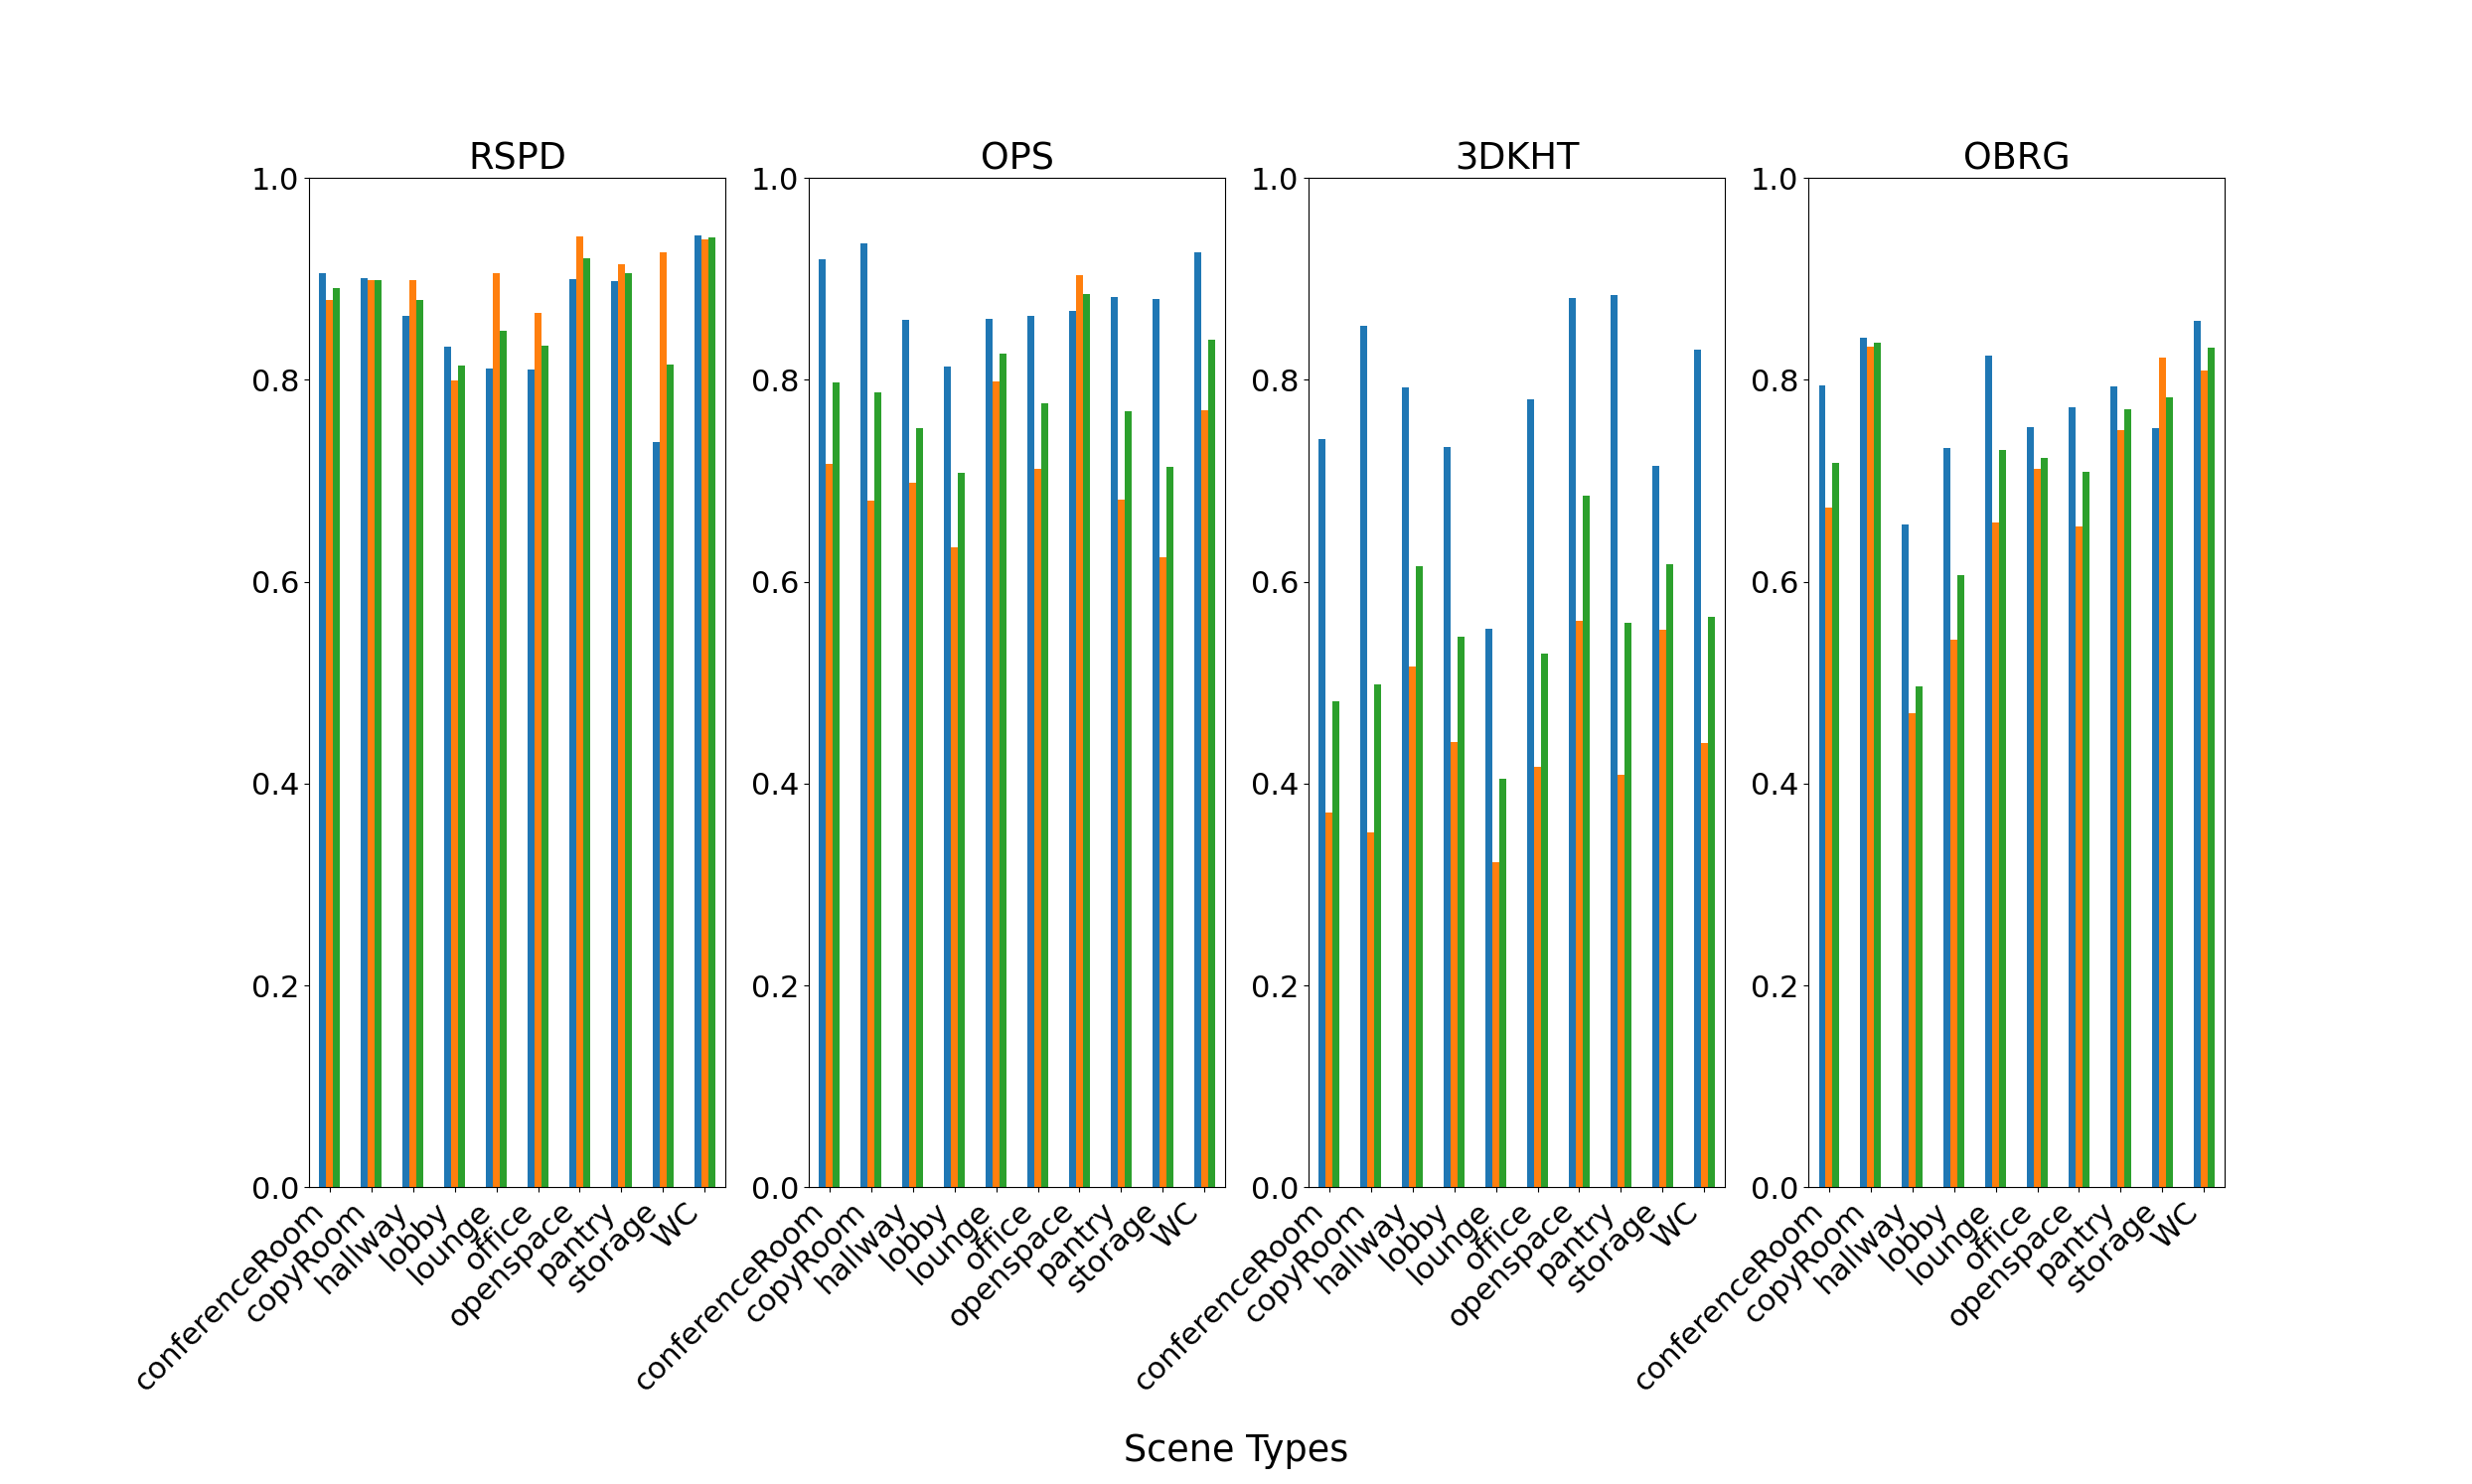
\includegraphics[width=\textwidth]{images/accuracy_total.png}
    \caption[Accuracy Results 2D-3D-S]{Average Accuracy for each scene type. The Precision
        is colored blue, recall is orange and the F1-score is green.}
    \label{fig:stanfordaccuracy}
\end{figure}

\begin{figure}[H]
    \centering
    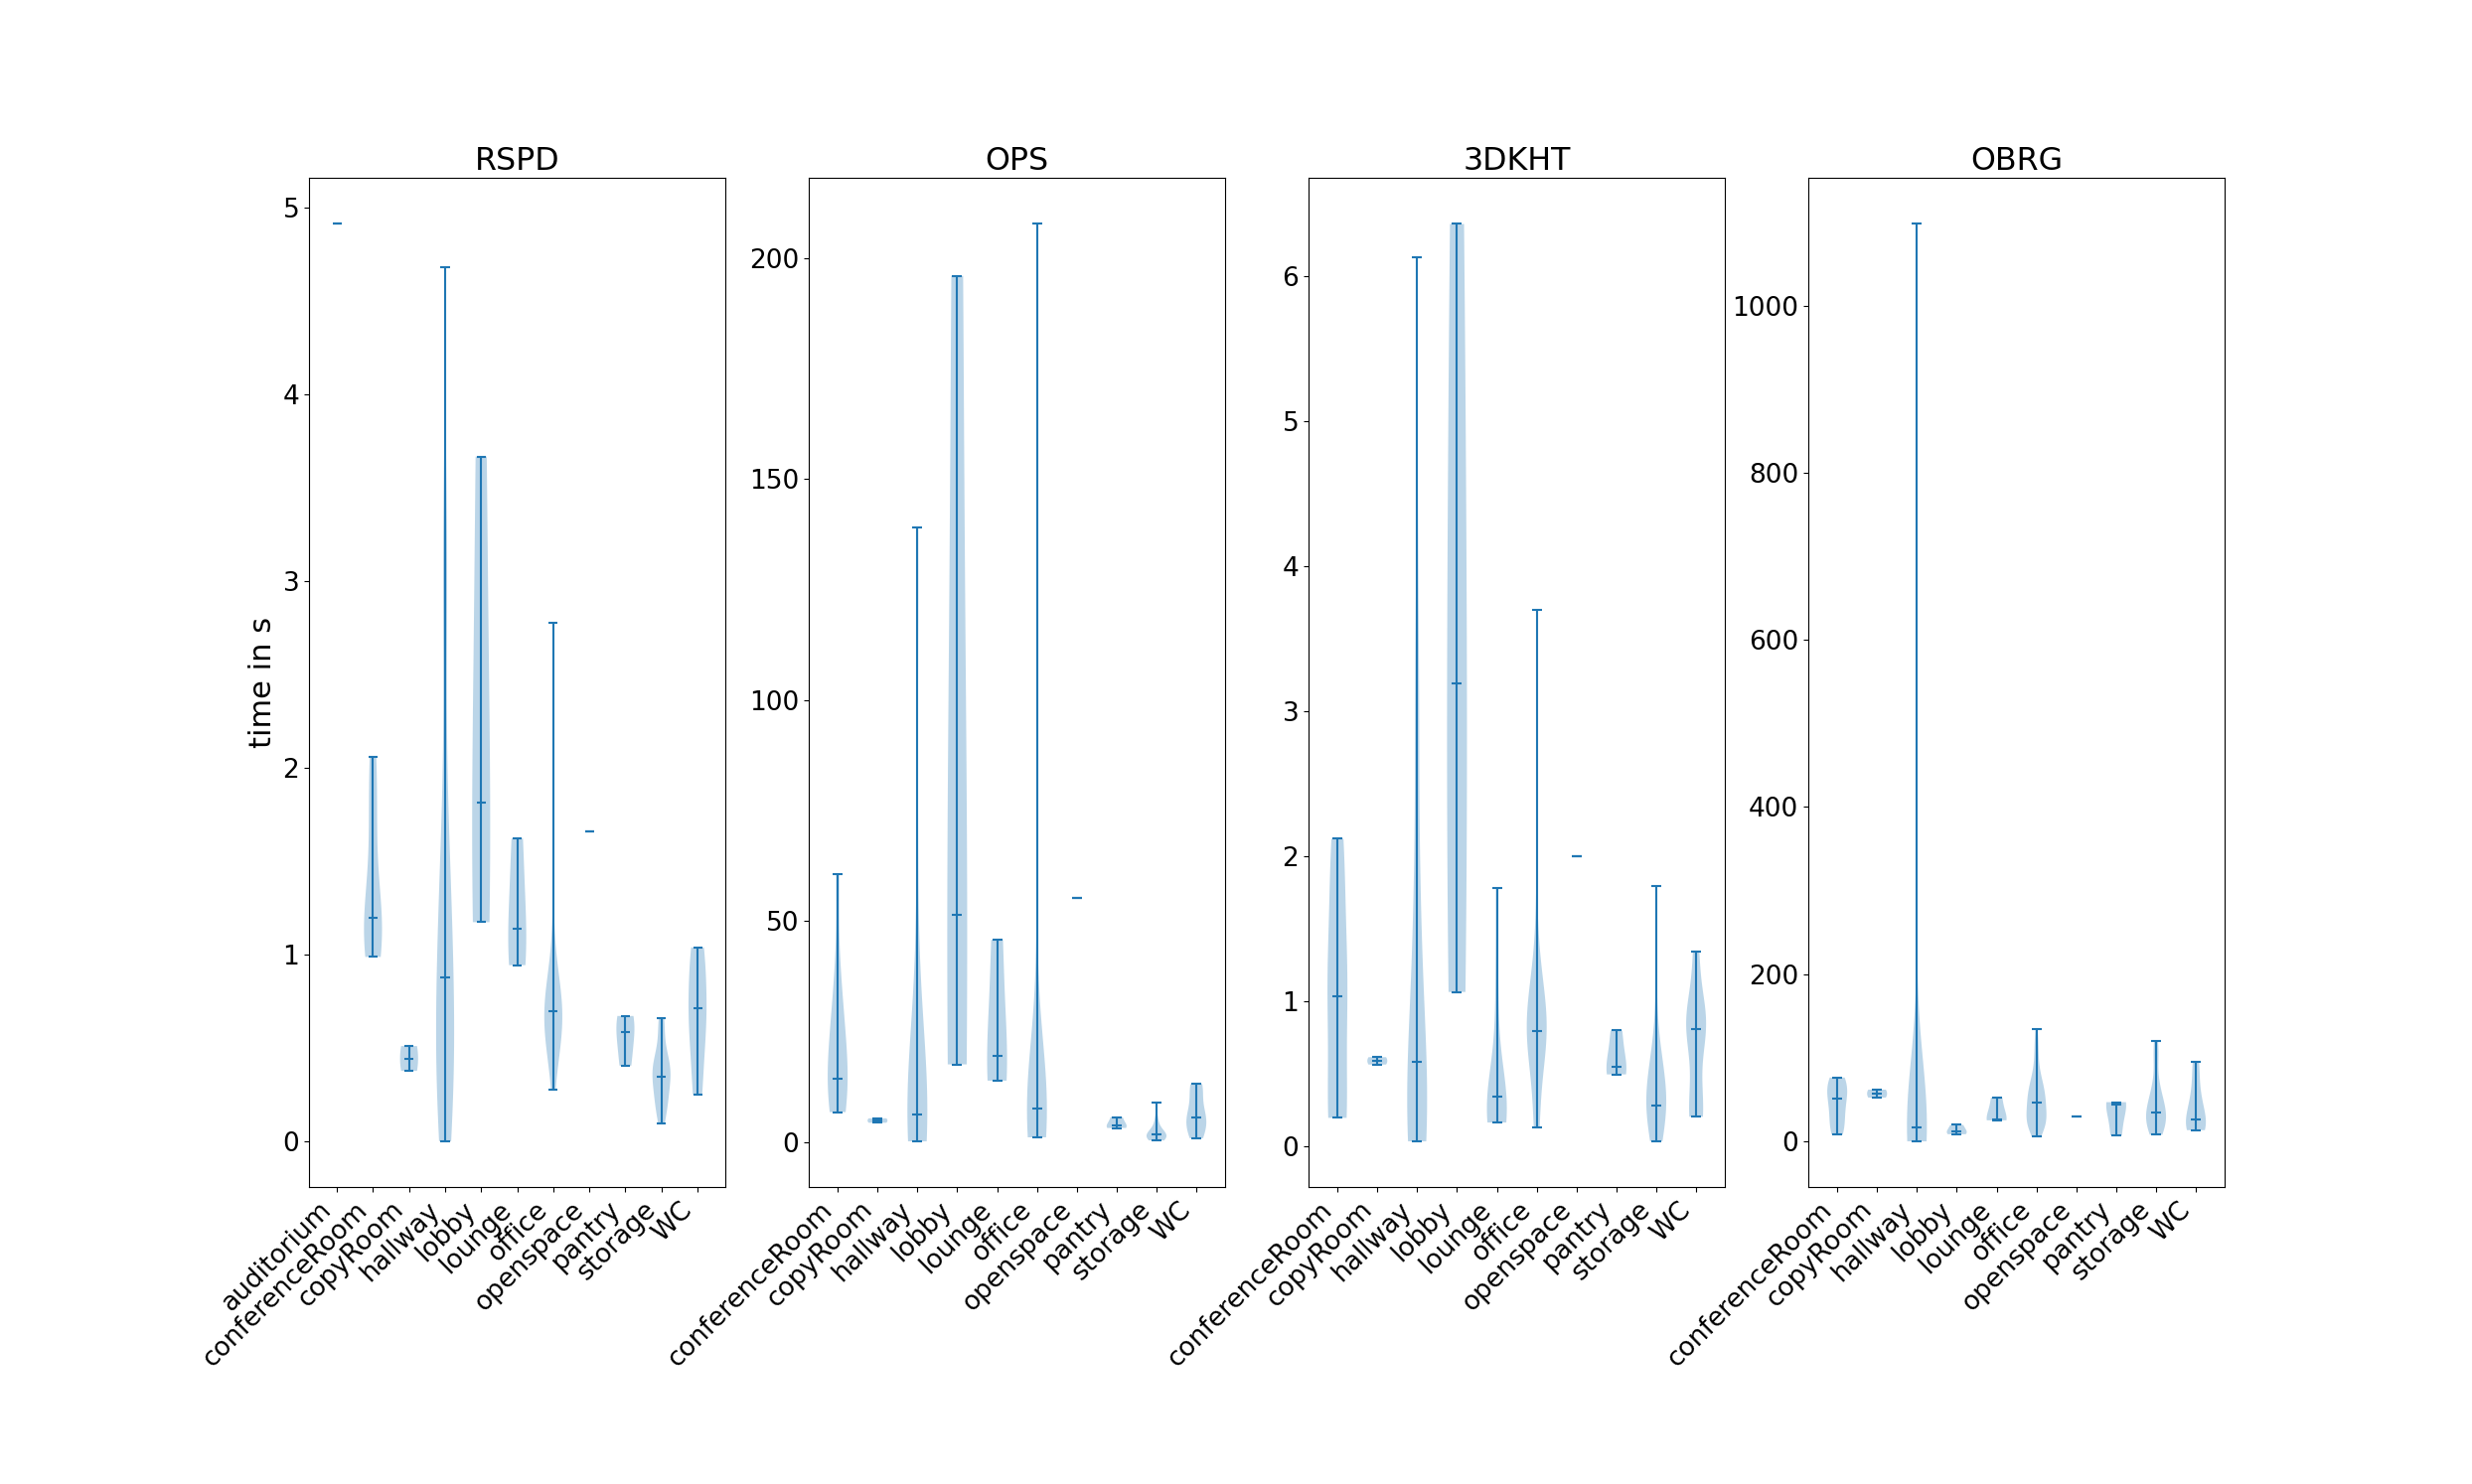
\includegraphics[width=15 cm]{images/times_violin.png}
    \caption[Time Results 2D-3D-S]{Times per scene type. The lowest tick denotes the minimum time, the highest
        denotes the maximum time spent in the calculation. The middle tick shows the mean time.
        Note, that the plots
        do not share the same y-axis.}
    \label{fig:violintime}
\end{figure}

\subsection{Results FIN Experiment}
\textit{So far:}
% FIXME lesbarkeit der figures!!!!
\begin{figure}[H]
    \centering
    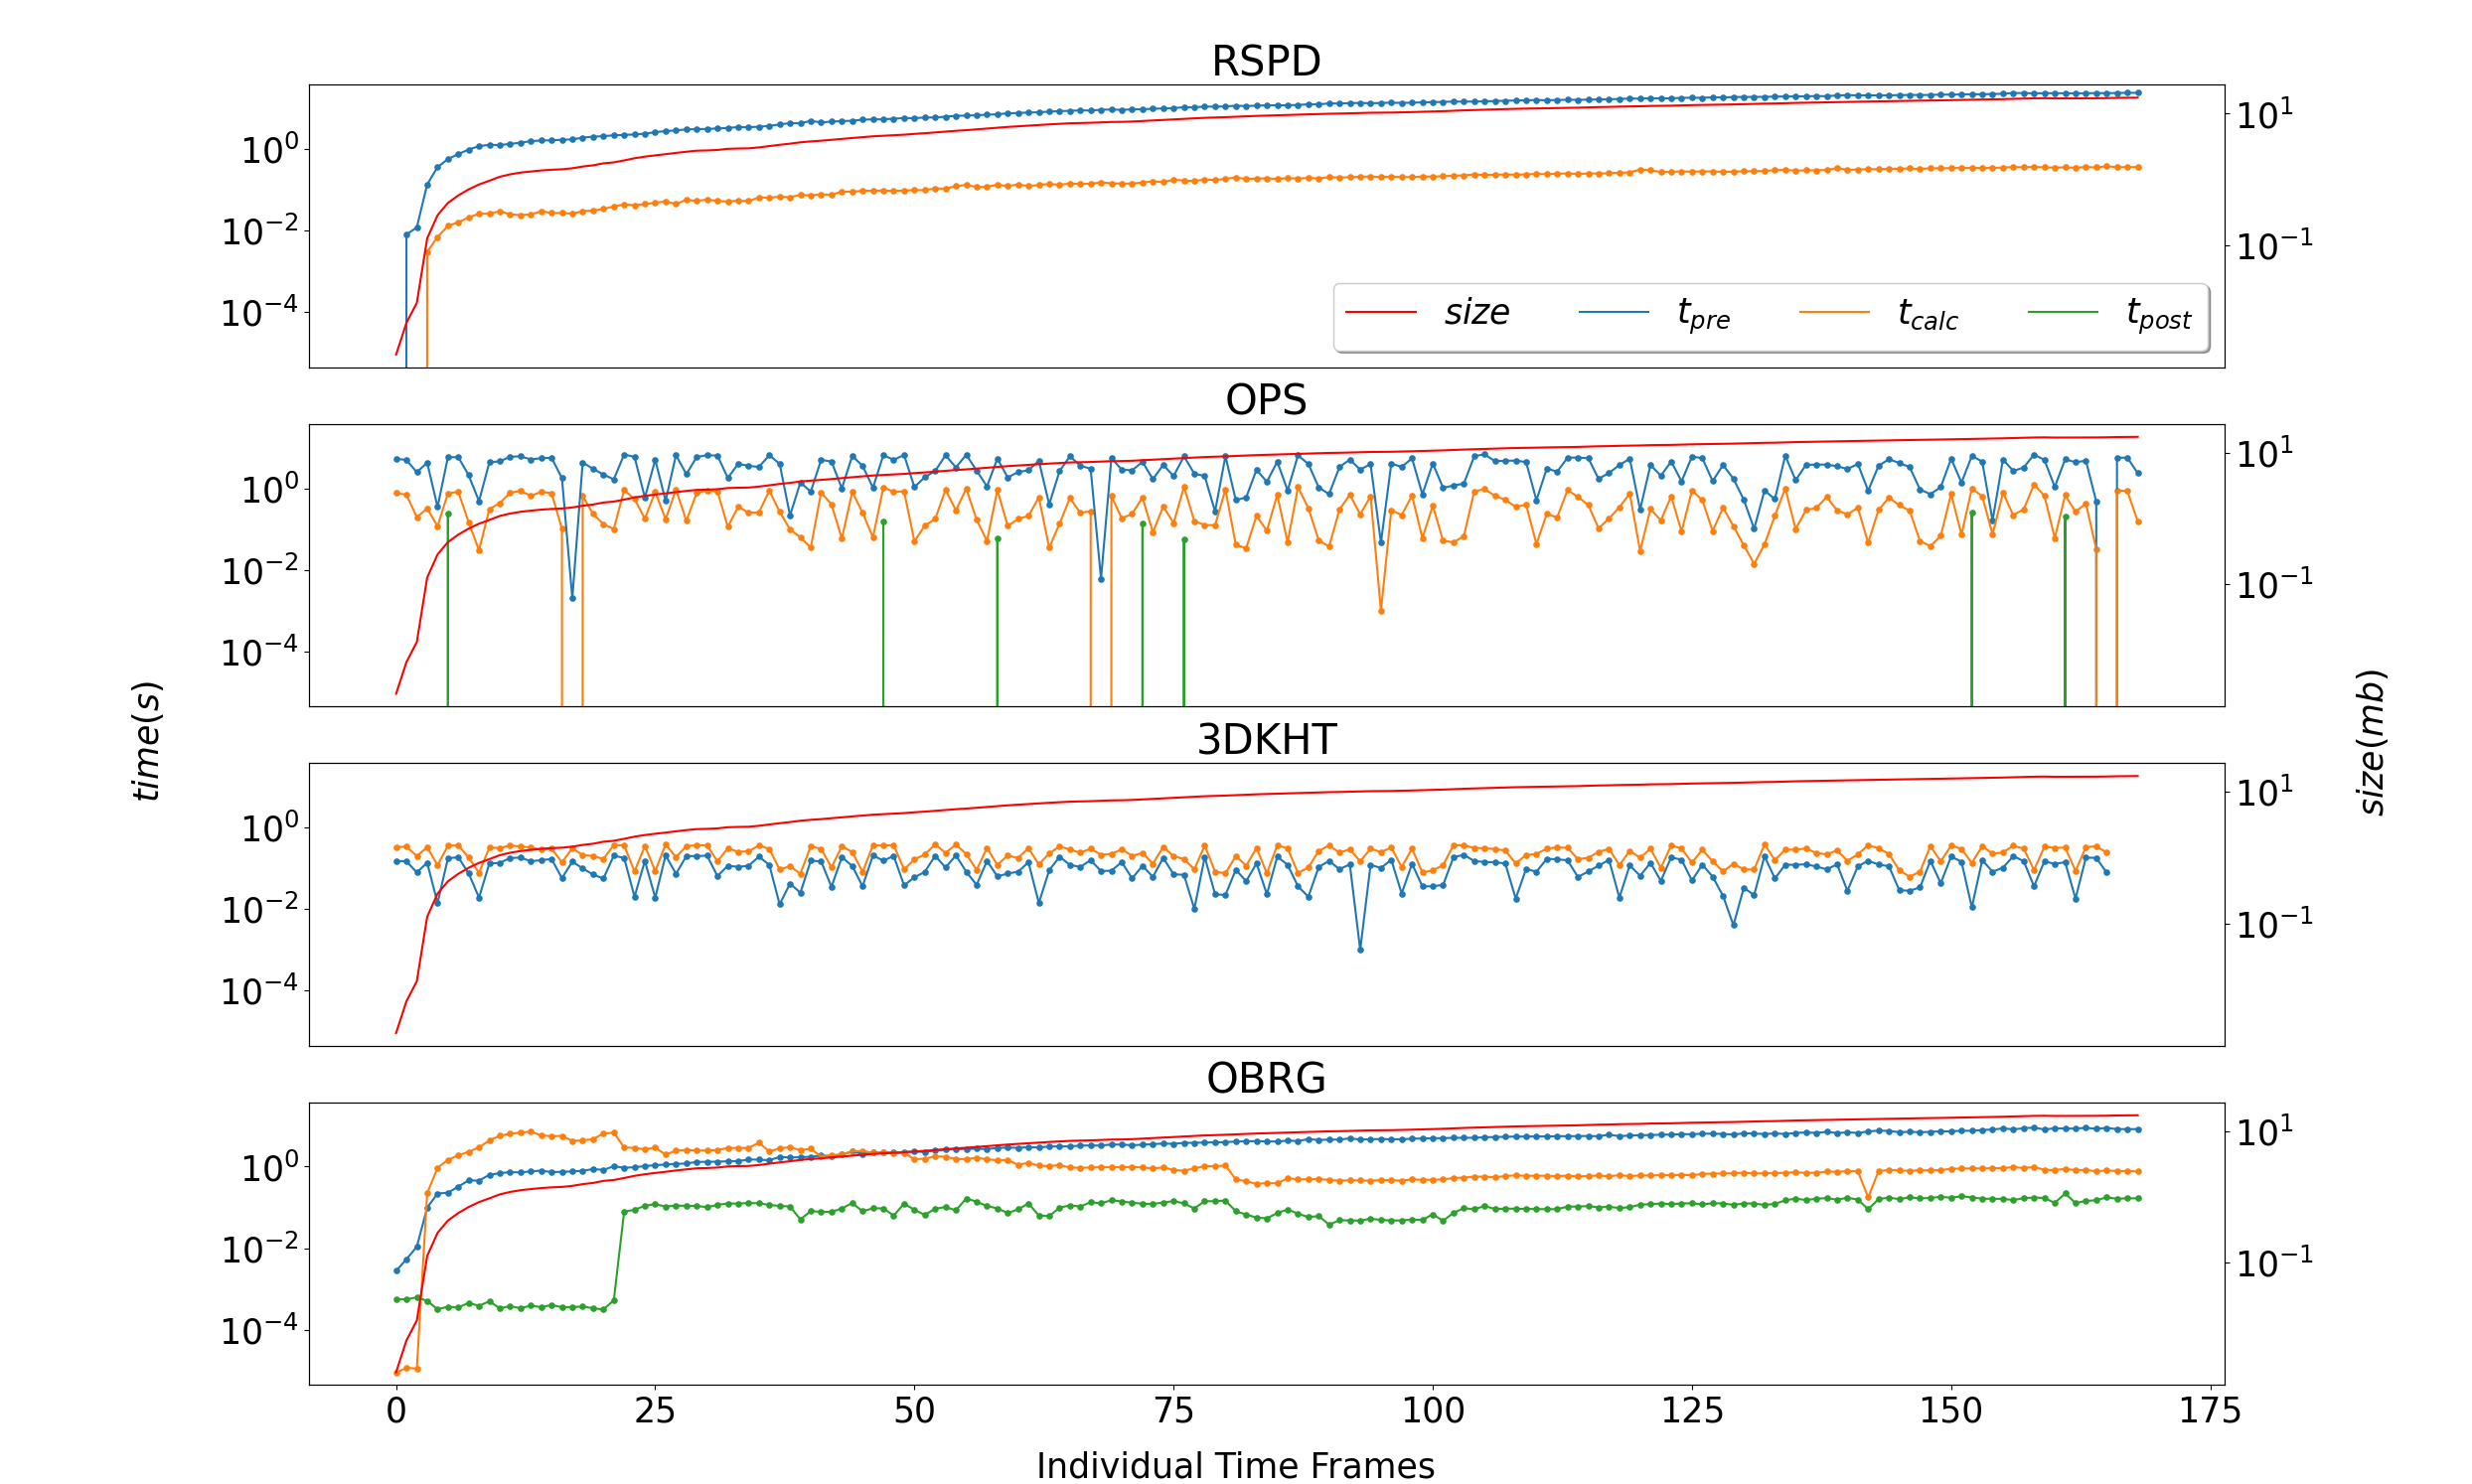
\includegraphics[width=0.8\textwidth]{images/dyn_time-hallway.png}
    \caption[Time Results Hallway]{Time spent in pre-processing (yellow), plane detection (blue), and post-processing (green) of the hallway scene and cloud sizes (red) of each time step.}
    \label{fig:dynhallway}
\end{figure}

\begin{figure}[H]
    \centering
    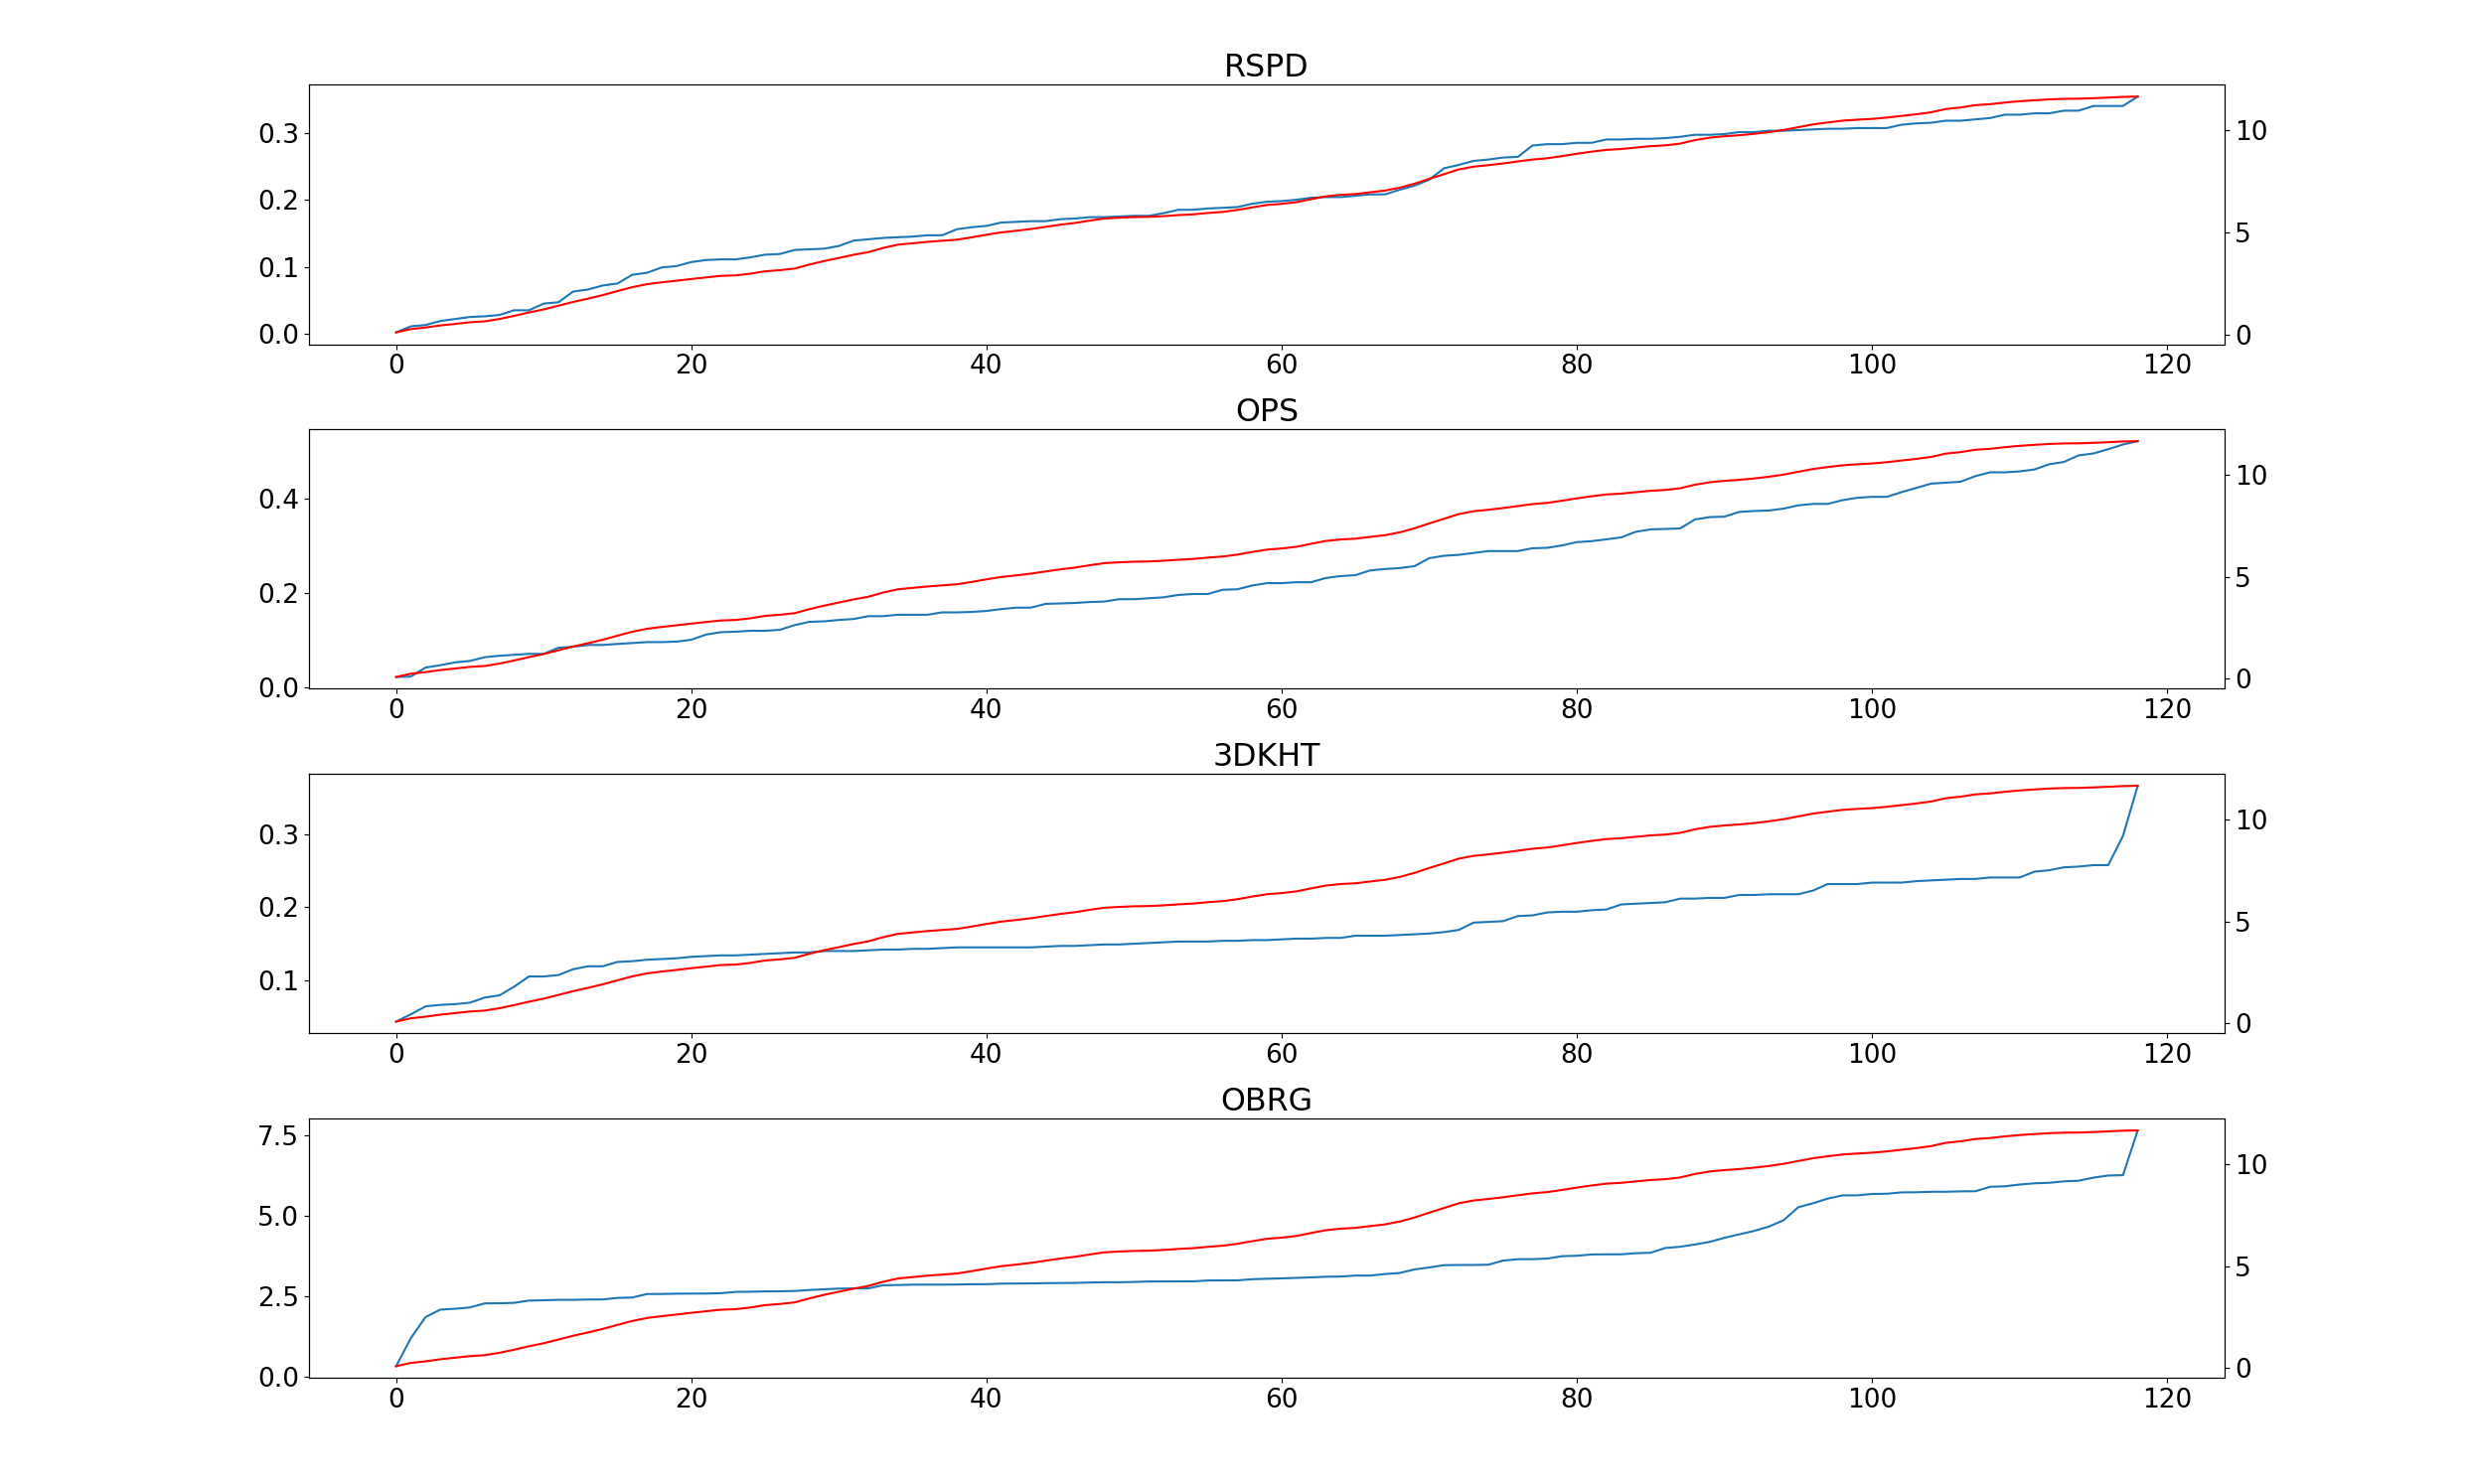
\includegraphics[width=0.8\textwidth]{images/dyn_time-office.png}
    \caption[Time Results office]{Time spent in pre-processing (yellow), plane detection (blue), and post-processing (green) of the office scene and cloud sizes (red) of each time step.}
    \label{fig:dynoffice}
\end{figure}

The calculation times of all algorithms except OBRG seem to be proportional to the size of the point cloud.
% TODO similar figure for 2D-3D-S
The quality of plane detection, however, decreases dramatically in comparison to the Stanford Datasets. RSPD is the only dataset that
is able to detect planes. %(see Figure~\ref{fig:}). 

% FIXME RERUN RSPD, OPS for time
% FIXME RERUN OBRG on all except office, conferenceroom 
\begin{table}[H]
    \centering
    \begin{tabular}{c|cccccc}
        Results FIN & Precision & Recall & F1-Score & $t_{pre}$ & $t_{calc}$ & $t_{post}$ \\ \hline
        RSPD        & 0.51      & 0.56   & 0.54     &           &            & /          \\
        OPS         & 0.69      & 0.29   & 0.39     & 1.14      & 21.23      & $<0.1$     \\
        3DKHT       & 0.49      & 0.44   & 0.46     & 0.14      & 0.29       & /          \\
        OBRG        & 0.492     & 0.274  & 0.339    & 4.91      & 37.50      & 0.10
    \end{tabular}
    \caption[Overall 2D-3D-S Results]{Average results of each algorithm over the FIN dataset. The right half of the columns shows the average time spent in
        pre-processing ($t_{pre}$), the average time spent in the plane detection itself ($t_{calc}$), and the average time spent in post-processing steps ($t_{post}$).
        Note, that the absence of post-processing steps is denoted as "/".}
    \label{tab:res-fin-total}
\end{table}

\textcolor{red}{Average zeiten bei einem wachsenden datensatz sind sinnlos.. oder? da finde ich macht die korrelation zwischen größe
    der punktwolke und dauer der berechnung mehr sinn}


\begin{table}[]
    \centering
    \begin{tabular}{c|cccccc}
               & Precision       & Recall          & F1-Score        \\ \hline
        RSPD   & 38.9\%          & \textbf{50.4\%} & \textbf{43.8\%} \\
        OPS    & 47.1\%          & 30.5\%          & 36.8\%          \\
        3D-KHT & 32.0\%          & 32.4\%          & 31.9\%          \\
        OBRG   & \textbf{50.8\%} & 34.5\%          & 40.6\%
    \end{tabular}%
    \caption{Average Results for the auditorium scene of the FIN dataset.}
    \label{tab:res-fin-audi}
\end{table}

\begin{table}[]
    \centering
    \begin{tabular}{c|cccccc}
               & Precision       & Recall          & F1-Score        & $t_{pre}$             & $t_{calc}$            & $t_{post}$            \\ \hline
        RSPD   & 58.2\%          & \textbf{63.2\%} & \textbf{60.5\%} & \textcolor{red}{todo} & \textcolor{red}{todo} & \textcolor{red}{todo} \\
        OPS    & \textbf{69.9\%} & 28.8\%          & 39.9\%          & \textcolor{red}{todo} & \textcolor{red}{todo} & \textcolor{red}{todo} \\
        3D-KHT & 47.4\%          & 45.9\%          & 46.2\%          & 0.21                  & 0.42                  & /                     \\
        OBRG   & 38.8\%          & 28.5\%          & 32.7\%          & 8.13                  & 117.72                & 0.65
    \end{tabular}%
    \caption{Average Results for the conferenceRoom scene of the FIN dataset.}
    \label{tab:res-fin-conf}
\end{table}

\begin{table}[]
    \centering
    \begin{tabular}{c|ccc}
               & Precision & Recall & F1-Score \\ \hline
        RSPD   & 0.50      & 0.51   & 0.51     \\
        OPS    & 0.87      & 0.20   & 0.32     \\
        3D-KHT & 0.57      & 0.44   & 0.49     \\
        OBRG   & 0.604     & 0.192  & 0.284
    \end{tabular}%
    \caption{Average Results for the hallway scene of the FIN dataset.}
    \label{tab:res-fin-hall}
\end{table}

\begin{table}[]
    \centering
    \begin{tabular}{c|ccc}
               & Precision       & Recall          & F1-Score        \\ \hline
        RSPD   & 71.1\%          & \textbf{69.9\%} & \textbf{70.4\%} \\
        OPS    & \textbf{74.7\%} & 37.1\%          & 49.2\%          \\
        3D-KHT & 62.3\%          & 54.9\%          & 58.2\%          \\
        OBRG   & 46.8\%          & 27.3\%          & 34.0\%
    \end{tabular}
    \caption{Average Results for the office scene of the FIN dataset.}
    \label{tab:res-fin-off}
\end{table}

\subsection{Summary Results}
% NOTE 3DKHT kann keine löcher oder non-rectangular ebenen basteln!
This section combines the preceding results of both experiments.
RSPD is the only algorithm that produces comparable results to the Stanford experiment in the dynamic experiment.
The remaining algorithms cannot reliably detect planes in an incrementally growing environment inheriting varying degrees of noise.

The reason for RSPD's dominance is likely caused by the inherent robustness against noise, as described in Section~

Die ergebnisse der beiden experimente unterscheiden sich in folgendem punkt. Dazu sei gesagt, dass die experimente folgende übereinstimmungen haben.
Das lässt sich so erklären. Alternative gründe davon könnten diese hier sein.

Ich denke RSPD ragt heraus, da hier besonders auf noise resistenz geachtet wurde. % TODO verweis auf diverse noise tests im BG


\end{document}